% answers.tex —— 2001 年·上海卷·文科 · 参考答案与详细解析片段
% 由 tools/generate_projects.py 依来源总账自 2001/2001_数学真题_上海文_试题.md + 2001/2001_数学真题_上海文_解析正文.md + 2001/2001_数学真题_上海文_答案要点.md 生成，勿手改（改源 MD 后重跑）


\begin{gktip}
固定源 PDF 为印刷页码 92–93 的两页题面，不附答案。以下解析均依据题面独立复算；第 12、19、22 题的图形在 LaTeX 工程中以 TikZ/PGFPlots 矢量源重绘。
\end{gktip}

\gkpart{一、填空题}

\begin{answer}
\gksolhead{1}{}

\textbf{题目}：

设函数 $f(x)=\log_9x$，则满足 $f(x)=\dfrac12$ 的 $x$ 值为\gkblank{}。

\Needspace{4\baselineskip}
\textbf{解析}

由 $\log_9x=\dfrac12$，得 $x=9^{1/2}=3$。

\gkanswer{答案：$3$}

\end{answer}
\begin{answer}
\gksolhead{2}{}

\textbf{题目}：

\Needspace{5\baselineskip}
设数列 $\{a_n\}$ 的首项 $a_1=-7$，且满足 $a_{n+1}=a_n+2$（$n\in\mathbb N$），则

\nopagebreak[4]
\[
a_1+a_2+\cdots+a_{17}=\_\_\_\_\_\_
\]

\Needspace{4\baselineskip}
\textbf{解析}

\Needspace{5\baselineskip}
这是首项 $a_1=-7$、公差 $d=2$ 的等差数列，因此

\nopagebreak[4]
\[
S_{17}=\frac{17}{2}\left[2(-7)+16\cdot2\right]=153.
\]

\gkanswer{答案：$153$}

\end{answer}
\begin{answer}
\gksolhead{3}{}

\textbf{题目}：

设 $P$ 为双曲线 $\dfrac{x^2}{4}-y^2=1$ 上一动点，$O$ 为坐标原点，$M$ 为线段 $OP$ 的中点，则点 $M$ 的轨迹方程为\gkblank{}。

\Needspace{4\baselineskip}
\textbf{解析}

\Needspace{5\baselineskip}
设 $M(x,y)$，则 $P(2x,2y)$。由于 $P$ 在双曲线上，

\nopagebreak[4]
\[
\frac{(2x)^2}{4}-(2y)^2=1,
\]

\Needspace{5\baselineskip}
化简得点 $M$ 的轨迹方程

\nopagebreak[4]
\[
x^2-4y^2=1.
\]

\gkanswer{答案：$x^2-4y^2=1$}

\end{answer}
\begin{answer}
\gksolhead{4}{}

\textbf{题目}：

设集合 $A=\{x\mid 2\lg x=\lg(8x-15),\ x\in\mathbb R\}$，$B=\left\{x\mid x\cos\dfrac{x}{2}>0,\ x\in\mathbb R\right\}$，则 $A\cap B$ 的元素个数为\gkblank{}个。

\Needspace{4\baselineskip}
\textbf{解析}

\Needspace{5\baselineskip}
由定义域和对数运算，

\nopagebreak[4]
\[
2\lg x=\lg(x^2)=\lg(8x-15),
\]

所以 $(x-3)(x-5)=0$，并结合定义域得 $A=\{3,5\}$。

\Needspace{5\baselineskip}
集合 $B$ 由 $x\cos(x/2)>0$ 给出。$3\cos(3/2)>0$，而 $5\cos(5/2)<0$，故

\nopagebreak[4]
\[
A\cap B=\{3\},
\]

元素个数为 $1$。

\gkanswer{答案：$1$}

\end{answer}
\begin{answer}
\gksolhead{5}{}

\textbf{题目}：

抛物线 $x^2-4y-3=0$ 的焦点坐标为\gkblank{}。

\Needspace{4\baselineskip}
\textbf{解析}

\nopagebreak[4]
\[
x^2-4y-3=0
\Longleftrightarrow x^2=4\left(y+\frac34\right).
\]

\Needspace{5\baselineskip}
抛物线顶点为 $(0,-3/4)$，焦参数为 $1$，故焦点为

\nopagebreak[4]
\[
\left(0,\frac14\right).
\]

\gkanswer{答案：$\left(0,\dfrac14\right)$}

\end{answer}
\begin{answer}
\gksolhead{6}{}

\textbf{题目}：

设数列 $\{a_n\}$ 是公比 $q>0$ 的等比数列，$S_n$ 是它的前 $n$ 项和。$\displaystyle\lim_{n\to\infty}S_n=7$，则此数列的首项 $a_1$ 的取值范围是\gkblank{}。

\Needspace{4\baselineskip}
\textbf{解析}

\Needspace{5\baselineskip}
因 $q>0$ 且 $S_n$ 有有限极限，故 $0<q<1$。由

\nopagebreak[4]
\[
\frac{a_1}{1-q}=7
\]

得 $a_1=7(1-q)$，所以 $a_1\in(0,7)$。

\gkanswer{答案：$(0,7)$}

\end{answer}
\begin{answer}
\gksolhead{7}{}

\textbf{题目}：

某餐厅供应客饭，每位顾客可以在餐厅提供的菜肴中任选 2 荤 2 素共 4 种不同的品种。现在餐厅准备了 5 种不同的荤菜，若要保证每位顾客有 200 种以上不同的选择，则餐厅至少还需要准备不同的素菜品种\gkblank{}种。（结果用数值表示）

\Needspace{4\baselineskip}
\textbf{解析}

\Needspace{5\baselineskip}
若素菜有 $n$ 种，选择数为

\nopagebreak[4]
\[
\binom52\binom n2=10\binom n2.
\]

要求 $10\binom n2\ge200$，即 $n(n-1)\ge40$。最小整数解为 $n=7$。

\gkanswer{答案：$7$}

\end{answer}
\begin{answer}
\gksolhead{8}{}

\textbf{题目}：

\Needspace{5\baselineskip}
在代数式

\nopagebreak[4]
\[
\left(x-\frac1{x^2}\right)^5
\]

的展开式中，常数项为\gkblank{}。

\Needspace{4\baselineskip}
\textbf{解析}

\Needspace{5\baselineskip}
展开通项为

\nopagebreak[4]
\[
(-1)^k\binom5k x^{5-3k},\qquad k=0,1,\ldots,5.
\]

常数项要求 $5-3k=0$，但 $k$ 不是整数，因此常数项为 $0$。

\gkanswer{答案：$0$}

\end{answer}
\begin{answer}
\gksolhead{9}{}

\textbf{题目}：

设 $x=\sin\alpha$，$\alpha\in\left[-\dfrac\pi6,\dfrac{5\pi}6\right]$，则 $\arccos x$ 的取值范围为\gkblank{}。

\Needspace{4\baselineskip}
\textbf{解析}

\Needspace{5\baselineskip}
在 $\alpha\in[-\pi/6,5\pi/6]$ 上，$\sin\alpha$ 的值域为 $[-1/2,1]$。所以

\nopagebreak[4]
\[
\arccos(\sin\alpha)\in
\left[0,\arccos\left(-\frac12\right)\right]
=\left[0,\frac{2\pi}{3}\right].
\]

\gkanswer{答案：$\left[0,\dfrac{2\pi}{3}\right]$}

\end{answer}
\begin{answer}
\gksolhead{10}{}

\textbf{题目}：

利用下列盈利表中的数据进行决策，应选择的方案是\gkblank{}。

\begin{center}
\begin{tabular}{lrrrrr}
\toprule
自然状况 & 概率 & $A_1$ & $A_2$ & $A_3$ & $A_4$ \\
\midrule
$S_1$ & $0.25$ & $50$ & $70$ & $-20$ & $98$ \\
$S_2$ & $0.30$ & $65$ & $26$ & $52$ & $82$ \\
$S_3$ & $0.45$ & $26$ & $16$ & $78$ & $-10$ \\
\bottomrule
\end{tabular}
\end{center}

\Needspace{4\baselineskip}
\textbf{解析}

\Needspace{5\baselineskip}
各方案的期望盈利为

\nopagebreak[4]
\[
\begin{aligned}
E(A_1)&=43.7,\\
E(A_2)&=32.5,\\
E(A_3)&=45.7,\\
E(A_4)&=44.6.
\end{aligned}
\]

所以应选择 $A_3$。

\gkanswer{答案：$A_3$}

\end{answer}
\begin{answer}
\gksolhead{11}{}

\textbf{题目}：

\Needspace{5\baselineskip}
已知两个圆：

\nopagebreak[4]
\[
x^2+y^2=1\quad(1),\qquad x^2+(y-3)^2=1\quad(2),
\]

则由（1）式减去（2）式可得上述两圆的对称轴方程。将上述命题在曲线的情况下加以推广，即要求得到一个更一般的命题，而已知命题应成为所推广命题的一个特例，推广的命题为\gkblank{}。

\Needspace{4\baselineskip}
\textbf{解析}

\Needspace{5\baselineskip}
设两圆的一般方程为

\nopagebreak[4]
\[
x^2+y^2+u_1x+v_1y+w_1=0,\qquad
x^2+y^2+u_2x+v_2y+w_2=0.
\]

\Needspace{5\baselineskip}
两式相减得到

\nopagebreak[4]
\[
(u_1-u_2)x+(v_1-v_2)y+(w_1-w_2)=0.
\]

该直线是两圆上点的幂相等的轨迹，即两圆的根轴；两圆相交时，它是公共弦所在直线。

\gkanswer{答案：两圆方程相减得到的方程表示两圆的根轴，即两圆上幂相等的点的轨迹；相交时为公共弦所在直线。}

\end{answer}
\begin{answer}
\gksolhead{12}{}

\textbf{题目}：

据报道，我国目前已成为世界上受荒漠化危害最严重的国家之一。下左图表示我国土地沙化总面积在上个世纪五六十年代、七八十年代、九十年代的变化情况。由图中的相关信息，可将上述有关年代中，我国年平均土地沙化面积在下右图中图示为：
\nopagebreak[4]
\begin{center}% 2001 年上海卷文科第 12 题：土地沙化面积与年平均变化量
\begin{tikzpicture}[>=stealth, scale=0.78]
  \begin{scope}
    \draw[->] (0,0)--(5.8,0) node[right] {年份};
    \draw[->] (0,0)--(0,3.2) node[above] {总面积};
    \draw[step=1cm, gray!25] (0,0) grid (5,3);
    \draw[thick] (0,0.25)--(2,1.05)--(4,2.05)--(5,2.7);
    \foreach \x/\label in {0/1950,1/1960,2/1970,3/1980,4/1990,5/2000}
      \node[below] at (\x,-0.08) {\scriptsize \label};
    \foreach \y/\label in {0.25/250.1,1.05/253.3,2.05/257.5,2.7/260}
      \node[left] at (-0.08,\y) {\scriptsize \label};
    \node[above] at (2.6,3.15) {\scriptsize 土地沙化总面积};
    \node[above] at (2.6,2.82) {\scriptsize （万平方公里）};
  \end{scope}
  \begin{scope}[xshift=7.1cm]
    \draw[->] (0,0)--(5.8,0) node[right] {年份};
    \draw[->] (0,0)--(0,3.2) node[above] {年平均};
    \draw[step=1cm, gray!25] (0,0) grid (5,3);
    \foreach \x/\label in {0/1950,1/1960,2/1970,3/1980,4/1990,5/2000}
      \node[below] at (\x,-0.08) {\scriptsize \label};
    \foreach \y/\label in {0.35/10,1.05/14,1.75/18,2.45/22,3/26}
      \node[left] at (-0.08,\y) {\scriptsize \label};
    \node[above] at (2.6,3.15) {\scriptsize 年平均土地沙化总面积};
    \node[above] at (2.6,2.82) {\scriptsize （百平方公里）};
  \end{scope}
\end{tikzpicture}
\end{center}
\nopagebreak[4]
\Needspace{4\baselineskip}
\textbf{解析}

\Needspace{5\baselineskip}
由左图数据，相关年代的总面积增量分别为

\nopagebreak[4]
\[
253.3-250.1=3.2,\quad
257.5-253.3=4.2,\quad
260-257.5=2.5.
\]

\Needspace{5\baselineskip}
按对应的 20 年、20 年、10 年区间计算，并将万平方公里换成百平方公里，年平均值为

\nopagebreak[4]
\[
16,\qquad 21,\qquad 25.
\]

因此应在右图网格对应的年代位置标出这三个数值并连接成折线；题面图的左侧数据与右侧待绘网格已在矢量源中重绘。

\gkanswer{答案：按题面数据在右图网格中绘制对应的年平均土地沙化面积图，见矢量图源。}

\end{answer}
\gkpart{二、选择题}

\begin{answer}
\gksolhead{13}{}

\textbf{题目}：

$a=3$ 是直线 $ax+2y+3a=0$ 和直线 $3x+(a-1)y=a-7$ 平行且不重合的\mbox{（　　）}

（A）充分非必要条件　　（B）必要非充分条件　　（C）充要条件　　（D）既非充分也非必要条件

\Needspace{4\baselineskip}
\textbf{解析}

\Needspace{5\baselineskip}
两直线平行需满足

\nopagebreak[4]
\[
\frac a3=\frac2{a-1},
\qquad a=3\ \text{\text{或}}\ a=-2.
\]

当 $a=3$ 时两直线为 $3x+2y+9=0$ 与 $3x+2y+4=0$，平行且不重合；当 $a=-2$ 时两式重合。因此条件“$a=3$”是题述条件的充要条件，选 C。

\gkanswer{答案：C}

\end{answer}
\begin{answer}
\gksolhead{14}{}

\textbf{题目}：

在平行六面体 $ABCD-A_1B_1C_1D_1$ 中，$M$ 为 $AC$ 与 $BD$ 的交点，若 $\overrightarrow{A_1B_1}=\boldsymbol a$、$\overrightarrow{A_1D_1}=\boldsymbol b$、$\overrightarrow{A_1A}=\boldsymbol c$，则下列向量中与 $\overrightarrow{B_1M}$ 相等的向量是\mbox{（　　）}

（A）$-\dfrac12\boldsymbol a+\dfrac12\boldsymbol b+\boldsymbol c$　　（B）$\dfrac12\boldsymbol a+\dfrac12\boldsymbol b+\boldsymbol c$

（C）$\dfrac12\boldsymbol a-\dfrac12\boldsymbol b+\boldsymbol c$　　（D）$-\dfrac12\boldsymbol a-\dfrac12\boldsymbol b+\boldsymbol c$

\Needspace{4\baselineskip}
\textbf{解析}

\Needspace{5\baselineskip}
取 $A_1$ 为原点，令 $B_1=\boldsymbol a$、$D_1=\boldsymbol b$、$A=\boldsymbol c$。平行六面体对角线交点为中点，所以

\nopagebreak[4]
\[
M=\boldsymbol c+\frac12(\boldsymbol a+\boldsymbol b).
\]

\Needspace{5\baselineskip}
于是

\nopagebreak[4]
\[
\overrightarrow{B_1M}
=-\frac12\boldsymbol a+\frac12\boldsymbol b+\boldsymbol c,
\]

选 A。

\gkanswer{答案：A}

\end{answer}
\begin{answer}
\gksolhead{15}{}

\textbf{题目}：

已知 $a$、$b$ 为两条不同的直线，$\alpha$、$\beta$ 为两个不同的平面，且 $a\perp\alpha$，$b\perp\beta$，则下列命题中的假命题是\mbox{（　　）}

（A）若 $a\parallel b$，则 $\alpha\parallel\beta$　　（B）若 $\alpha\perp\beta$，则 $a\perp b$

（C）若 $a$、$b$ 相交，则 $\alpha$、$\beta$ 相交　　（D）若 $\alpha$、$\beta$ 相交，则 $a$、$b$ 相交

\Needspace{4\baselineskip}
\textbf{解析}

平面相交时，其法向方向可以是异面直线，不能推出两条法向直线相交。因此 D 为假命题，选 D。

\gkanswer{答案：D}

\end{answer}
\begin{answer}
\gksolhead{16}{}

\textbf{题目}：

用计算器验算函数 $y=\dfrac{\lg x}{x}$（$x>1$）的若干个值，可以猜想下列命题中的真命题只能是\mbox{（　　）}

（A）$y=\dfrac{\lg x}{x}$ 在 $(1,+\infty)$ 上是单调减函数

（B）$y=\dfrac{\lg x}{x}$，$x\in(1,+\infty)$ 的值域为 $\left(0,\dfrac{\lg3}{3}\right]$

（C）$y=\dfrac{\lg x}{x}$，$x\in(1,+\infty)$ 有最小值

（D）$\displaystyle\lim_{n\to\infty}\dfrac{\lg n}{n}=0,\ n\in\mathbb N$

\Needspace{4\baselineskip}
\textbf{解析}

\Needspace{5\baselineskip}
函数 $\lg x/x$ 在 $x=e$ 附近先增后减，没有全程单调减，也没有最小值；其最大值也不是 $\lg3/3$。但

\nopagebreak[4]
\[
\lim_{n\to\infty}\frac{\lg n}{n}=0,
\]

故选 D。

\gkanswer{答案：D}

\end{answer}
\gkpart{三、解答题}

\begin{answer}
\gksolhead{17}{}

\textbf{题目}：

已知 $a\text{、}b\text{、}c$ 是 $\triangle ABC$ 中 $\angle A\text{、}\angle B\text{、}\angle C$ 的对边，$S$ 是 $\triangle ABC$ 的面积，若 $a=4$，$b=5$，$S=5\sqrt3$，求 $c$ 的长度。

\Needspace{4\baselineskip}
\textbf{解析}

\Needspace{5\baselineskip}
由

\nopagebreak[4]
\[
5\sqrt3=\frac12\cdot4\cdot5\sin C
\]

\Needspace{5\baselineskip}
得 $\sin C=\sqrt3/2$，所以 $C=60^\circ$ 或 $120^\circ$。余弦定理给出

\nopagebreak[4]
\[
c^2=4^2+5^2-2\cdot4\cdot5\cos C.
\]

\Needspace{5\baselineskip}
两种情形分别得到

\nopagebreak[4]
\[
c=\sqrt{21}\quad\text{\text{或}}\quad c=\sqrt{61}.
\]

\gkanswer{答案：$c=\sqrt{21}$ 或 $c=\sqrt{61}$。}

\end{answer}
\begin{answer}
\gksolhead{18}{}

\textbf{题目}：

设 $F_1\text{、}F_2$ 为椭圆 $\dfrac{x^2}{9}+\dfrac{y^2}{4}=1$ 的两个焦点，$P$ 为椭圆上的一点。已知 $P\text{、}F_1\text{、}F_2$ 是一个直角三角形的三个顶点，且 $|PF_1|>|PF_2|$，求 $\dfrac{|PF_1|}{|PF_2|}$ 的值。

\Needspace{4\baselineskip}
\textbf{解析}

\Needspace{5\baselineskip}
椭圆的焦半距为 $c=\sqrt{3^2-2^2}=\sqrt5$，所以 $|F_1F_2|=2\sqrt5$，且

\nopagebreak[4]
\[
r_1=|PF_1|,\quad r_2=|PF_2|,\quad r_1+r_2=6,\quad r_1>r_2.
\]

若直角在 $P$，则 $r_1^2+r_2^2=20$，从而 $r_1r_2=8$，得 $(r_1,r_2)=(4,2)$，比值为 $2$。

\Needspace{5\baselineskip}
若直角在 $F_1$，则 $r_2$ 为斜边，与 $r_1>r_2$ 矛盾；若直角在 $F_2$，则

\nopagebreak[4]
\[
r_1^2-r_2^2=20,\qquad r_1+r_2=6,
\]

所以 $r_1-r_2=10/3$，从而 $(r_1,r_2)=(14/3,4/3)$，比值为 $7/2$。

\Needspace{5\baselineskip}
故答案为

\nopagebreak[4]
\[
2\quad\text{\text{或}}\quad\frac72.
\]

\gkanswer{答案：$2$ 或 $\dfrac72$。}

\end{answer}
\begin{answer}
\gksolhead{19}{}

\textbf{题目}：

在棱长为 $a$ 的正方体 $OABC-O'A'B'C'$ 中，$E\text{、}F$ 分别是棱 $AB\text{、}BC$ 上的动点，且 $AE=BF$。
\nopagebreak[4]
\begin{center}% 2001 年上海卷文科第 19 题：正方体与动点
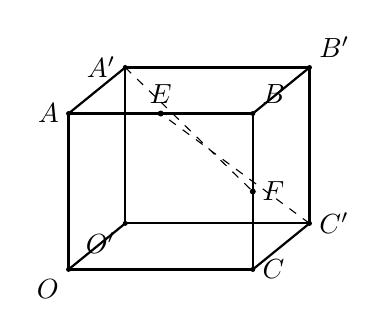
\begin{tikzpicture}[>=stealth, scale=0.9]
  \coordinate (O) at (0,0);
  \coordinate (A) at (0,2.2);
  \coordinate (B) at (2.6,2.2);
  \coordinate (C) at (2.6,0);
  \coordinate (O1) at (0.8,0.65);
  \coordinate (A1) at (0.8,2.85);
  \coordinate (B1) at (3.4,2.85);
  \coordinate (C1) at (3.4,0.65);
  \coordinate (E) at (1.3,2.2);
  \coordinate (F) at (2.6,1.1);

  \draw[thick] (O)--(A)--(B)--(C)--cycle;
  \draw[thick] (O1)--(A1)--(B1)--(C1)--cycle;
  \draw[thick] (O)--(O1) (A)--(A1) (B)--(B1) (C)--(C1);
  \draw[dashed] (A1)--(F) (C1)--(E);
  \fill (E) circle (1.2pt) node[above] {$E$};
  \fill (F) circle (1.2pt) node[right] {$F$};
  \fill (O) circle (1pt) node[below left] {$O$};
  \fill (A) circle (1pt) node[left] {$A$};
  \fill (B) circle (1pt) node[above right] {$B$};
  \fill (C) circle (1pt) node[right] {$C$};
  \fill (O1) circle (1pt) node[below left] {$O'$};
  \fill (A1) circle (1pt) node[left] {$A'$};
  \fill (B1) circle (1pt) node[above right] {$B'$};
  \fill (C1) circle (1pt) node[right] {$C'$};
\end{tikzpicture}
\end{center}
\nopagebreak[4]
（1） 求证：$A'F\perp C'E$；

（2） 当三棱锥 $B'-BEF$ 的体积取得最大值时，求二面角 $B'-EF-B$ 的大小。（结果用反三角函数表示）

\Needspace{4\baselineskip}
\textbf{解析}

\Needspace{5\baselineskip}
取

\nopagebreak[4]
\[
O=(0,0,0),\quad A=(0,a,0),\quad B=(a,a,0),\quad C=(a,0,0),
\]

\Needspace{5\baselineskip}
并设 $AE=BF=t$，则

\nopagebreak[4]
\[
E=(t,a,0),\quad F=(a,a-t,0),\quad
A'=(0,a,a),\quad C'=(a,0,a).
\]

\gksubpart{(1)}

\nopagebreak[4]
\[
\overrightarrow{A'F}=(a,-t,-a),\qquad
\overrightarrow{C'E}=(t-a,a,-a),
\]

\Needspace{5\baselineskip}
故

\nopagebreak[4]
\[
\overrightarrow{A'F}\cdot\overrightarrow{C'E}
=a(t-a)-at+a^2=0,
\]

所以 $A'F\perp C'E$。

\gksubpart{(2)}

\Needspace{5\baselineskip}
三棱锥体积为

\nopagebreak[4]
\[
V=\frac13\cdot\frac12t(a-t)\cdot a
=\frac16at(a-t),
\]

在 $t=a/2$ 时最大。

\Needspace{5\baselineskip}
令 $a=1$，此时平面 $BEF$ 为 $z=0$，平面 $B'EF$ 的法向量可取 $\boldsymbol n=(-2,-2,1)$。故二面角 $\varphi$ 满足

\nopagebreak[4]
\[
\cos\varphi=\frac13,\qquad \tan\varphi=2\sqrt2.
\]

\Needspace{5\baselineskip}
所以

\nopagebreak[4]
\[
\varphi=\arctan(2\sqrt2).
\]

\gkanswer{答案（1）：见解析。}

\gkanswer{答案（2）：二面角大小为 $\arctan(2\sqrt2)$。}

\end{answer}
\begin{answer}
\gksolhead{20}{}

\textbf{题目}：

\Needspace{5\baselineskip}
对任意一个非零复数 $z$，定义集合

\nopagebreak[4]
\[
M_z=\{\omega\mid \omega=z^{2n-1},\ n\in\mathbb N\}.
\]

（1） 设 $a$ 是方程 $x+\dfrac1x=2$ 的一个根，试用列举法表示集合 $M_a$。若在 $M_a$ 中任取两个数，求其和为零的概率 $P$；

（2） 设集合 $M_z$ 中只有 3 个元素，试写出满足条件的一个 $z$ 的值，并说明理由。

\Needspace{4\baselineskip}
\textbf{解析}

\gksubpart{(1)}

\nopagebreak[4]
\[
x+\frac1x=2
\Longleftrightarrow (x-1)^2=0,
\]

故 $a=1$，从而 $M_a=\{1\}$。任取其中两个数，其和为 $2$，所以 $P=0$。

\gksubpart{(2)}

\Needspace{5\baselineskip}
取 $z=e^{i\pi/3}$。其奇数次幂在模 $6$ 意义下只有 $1,3,5$ 三种指数，因此

\nopagebreak[4]
\[
M_z=\left\{e^{i\pi/3},-1,e^{i5\pi/3}\right\},
\]

恰有三个元素。

\gkanswer{答案（1）：$M_a=\{1\}$，$P=0$。}

\gkanswer{答案（2）：例如 $z=e^{i\pi/3}$。}

\end{answer}
\begin{answer}
\gksolhead{21}{}

\textbf{题目}：

用水清洗一堆蔬菜上残留的农药，对用一定量的水清洗一次的效果作如下假定：用 1 个单位量的水可洗掉蔬菜上残留农药用量的 $\dfrac12$，用水越多洗掉的农药量也越多，但总还有农药残留在蔬菜上。设用 $x$ 单位量的水清洗一次以后，蔬菜上残留的农药与本次清洗前残留的农药量之比为函数 $f(x)$。

（1） 试规定 $f(0)$ 的值，并解释其实际意义；

（2） 试根据假定写出函数 $f(x)$ 应该满足的条件和具有的性质；

（3） 设 $f(x)=\dfrac1{1+x^2}$，现有 $a$（$a>0$）单位量的水，可以清洗一次，也可以把水平均分成 2 份后清洗两次。试问用哪种方案清洗后蔬菜上的农药量比较少？说明理由。

\Needspace{4\baselineskip}
\textbf{解析}

\gksubpart{(1)}

不使用水时残留量不变，故 $f(0)=1$。

\gksubpart{(2)}

可取定义域为 $[0,+\infty)$。由假定，$f(0)=1$，$0<f(x)\le1$，且 $f$ 随 $x$ 增大而减小；总有残留量可表示为 $f(x)>0$，并可取 $\lim_{x\to+\infty}f(x)=0$。

\gksubpart{(3)}

\Needspace{5\baselineskip}
一次清洗后的残留比例为

\nopagebreak[4]
\[
R_1=\frac1{1+a^2}.
\]

\Needspace{5\baselineskip}
分两次清洗后的残留比例为

\nopagebreak[4]
\[
R_2=f\left(\frac a2\right)^2
=\frac1{\left(1+\frac{a^2}{4}\right)^2}.
\]

\Needspace{5\baselineskip}
比较可得

\nopagebreak[4]
\[
R_2<R_1\Longleftrightarrow a^2>8.
\]

所以 $a>2\sqrt2$ 时分两次较少，$a=2\sqrt2$ 时相同，$0<a<2\sqrt2$ 时一次清洗较少。

\gkanswer{答案（1）：$f(0)=1$，表示不使用水清洗时，清洗后残留量与清洗前相等。}

\gkanswer{答案（2）：可取定义域 $[0,+\infty)$；$f(0)=1$，$0<f(x)\le1$，且 $f$ 随 $x$ 增大而减小，通常还应有 $\displaystyle\lim_{x\to+\infty}f(x)=0$。}

\gkanswer{答案（3）：$0<a<2\sqrt2$ 时一次清洗较少；$a=2\sqrt2$ 时两种方案相同；$a>2\sqrt2$ 时分两次清洗较少。}

\end{answer}
\begin{answer}
\gksolhead{22}{}

\textbf{题目}：

对任意函数 $f(x)$，$x\in D$，可按图示构造一个数列发生器，其工作原理如下：

①输入数据 $x_0\in D$，经数列发生器输出 $x_1=f(x_0)$；

\Needspace{5\baselineskip}
②若 $x_1\notin D$，则数列发生器结束工作；若 $x_1\in D$，则将 $x_1$ 反馈回输入端，再输出 $x_2=f(x_1)$，并依此规律继续下去。现定义

\nopagebreak[4]
\[
f(x)=\frac{4x-2}{x+1}.
\]
\nopagebreak[4]
\begin{center}% 2001 年上海卷文科第 22 题：数列发生器流程图
\begin{tikzpicture}[>=stealth, node distance=0.6cm]
  \tikzset{box/.style={draw, minimum width=1.1cm, minimum height=0.55cm, align=center}}
  \node[box] (f) {$f$};
  \node[box, below=of f] (print) {打印};
  \node[box, below=of print, minimum width=1.8cm] (test) {$x_1\in D$};
  \node[below=of test] (end) {结束};
  \draw[->] (f)--node[right] {输出}(print);
  \draw[->] (print)--(test);
  \draw[->] (test)--node[right] {NO}(end);
  \draw[->] (test.east)--++(1.0,0)--++(0,2.0)--node[above] {YES} (f.east);
  \draw[->] ($(f.north)+(0,0.7)$)--node[left] {输入}(f.north);
\end{tikzpicture}
\end{center}
\nopagebreak[4]
（1） 若输出 $x_0=\dfrac{49}{65}$，则由数列发生器产生数列 $\{x_n\}$。请写出数列 $\{x_n\}$ 的所有项；

（2） 若要数列发生器产生一个无穷的常数数列，试求输出的初始数据 $x_0$ 的值；

（3） 是否存在 $x_0$，在输入数据 $x_0$ 时，该数列发生器产生一个各项均为负数的无穷数列？若存在，求出 $x_0$ 的值；若不存在，请说明理由。

\Needspace{4\baselineskip}
\textbf{解析}

函数的定义域为 $D=\mathbb R\setminus\{-1\}$。

\gksubpart{(1)}

\nopagebreak[4]
\[
x_1=f\left(\frac{49}{65}\right)=\frac{11}{19},\qquad
x_2=f\left(\frac{11}{19}\right)=\frac15,\qquad
x_3=f\left(\frac15\right)=-1.
\]

\Needspace{5\baselineskip}
由于 $-1\notin D$，发生器停止，所有输出项为

\nopagebreak[4]
\[
\frac{49}{65},\quad\frac{11}{19},\quad\frac15,\quad-1.
\]

\gksubpart{(2)}

\Needspace{5\baselineskip}
常数数列要求 $f(x_0)=x_0$，即

\nopagebreak[4]
\[
\frac{4x_0-2}{x_0+1}=x_0
\Longleftrightarrow x_0^2-3x_0+2=0.
\]

故 $x_0=1$ 或 $x_0=2$。

\gksubpart{(3)}

若 $f(x)<0$，则由分式符号得 $-1<x<1/2$；结合 $x<0$，必须有 $-1<x<0$。但此时 $f(x)<-2$，下一次代入小于 $-1$ 的数后，分子分母同为负，函数值变为正。因此不可能产生各项均为负的无穷数列。

\gkanswer{答案（1）：$\{x_n\}=\left\{\dfrac{49}{65},\dfrac{11}{19},\dfrac15,-1\right\}$，输出 $-1$ 后停止。}

\gkanswer{答案（2）：$x_0=1$ 或 $x_0=2$。}

\gkanswer{答案（3）：不存在这样的 $x_0$。}

\end{answer}